% 1959 年全国卷第 6 题：三条互不共面的平行线与四面体 ABCD。
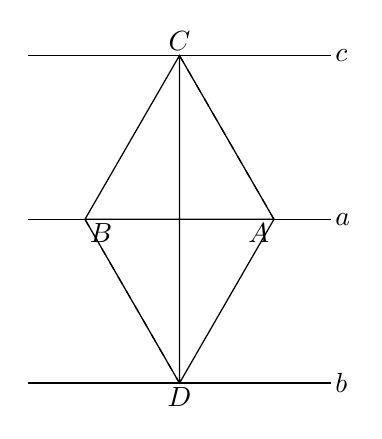
\begin{tikzpicture}[scale=0.8, line width=0.45pt,
  every node/.style={inner sep=1.5pt}]
  \coordinate (C) at (0,2.8); \coordinate (D) at (0,-2.4);
  \coordinate (B) at (-1.5,0.2); \coordinate (A) at (1.5,0.2);
  \draw (-2.4,2.8)--(2.4,2.8) node[anchor=west] {$c$};
  \draw (-2.4,0.2)--(2.4,0.2) node[anchor=west] {$a$};
  \draw (-2.4,-2.4)--(2.4,-2.4) node[anchor=west] {$b$};
  \draw (A)--(B)--(C)--cycle (A)--(D)--(B) (C)--(D);
  \draw[dashed] (C)--(A) (B)--(D);
  \draw[dashed] (C)--(D);
  \node[anchor=south] at (C) {$C$}; \node[anchor=north] at (D) {$D$};
  \node[anchor=north east] at (A) {$A$}; \node[anchor=north west] at (B) {$B$};
\end{tikzpicture}
